\documentclass{article}
%\usepackage{fullpage}
\usepackage{sidecap}
\usepackage{mathtools}
\usepackage{mhchem}
\usepackage{amssymb}
\usepackage{amsmath}
\usepackage{bm}
\usepackage{gensymb}
\usepackage{siunitx}
\usepackage{cancel}
\usepackage{graphicx}
\usepackage{subcaption}
\author{Mann, J}
\title{Day 2 Notes}
\date{September 1, 2015}
\renewcommand{\d}[0]{\mathrm{d}}
\newcommand{\pOne}[2]{\frac{\partial #1}{\partial #2}}
\renewcommand{\deg}[0]{\degree}
\newcommand{\pTwo}[2]{\frac{\partial^2 #1}{\partial #2^2}}
\newcommand{\dOne}[2]{\frac{\d #1}{\d #2}}
\newcommand{\dTwo}[2]{\frac{\d^2 #1}{\d #2^2}}
\newcommand{\diag}[1]{\bcancel{#1}}
\newcommand{\matr}[1]{\bm{#1}}
\graphicspath{{Day2NotesPics/}}
\begin{document}
\maketitle{}
\begin{section}{Introduction}
  Lecture 1 Structure: Thermodynamics

  See papers by 
  \begin{itemize}
    \item Hansen \{ 1962 \}
    \item Cahn
    \item Mann \& Turkevich
  \end{itemize}

  Copies are on Blackboard
\end{section}
\begin{section}{Surface Tension}
  \begin{align*}
    -\d\gamma = \bar{S}\d T - \tau \d P + \sum_{c=1}^{N}\Gamma_c \d \mu_c
  \end{align*}
  \begin{center}
    \begin{tabular}{|c|l|}
      \hline
      $T$ & Temperature\\
      $P$ & Pressure\\
      $\mu_c$ & chemical potential\\
      \hline
    \end{tabular}
  \end{center}
  
  Note the sign

  Given a uniform $T,P,\left\{ \mu_i \right\}$ develop a function relating 
  \begin{align*}
    \gamma=\gamma(T,P,\left\{ \mu_i \right\})
  \end{align*}
  Restriction: Gibb's phase rule:
  \begin{align*}
    \mathrm{\#\ degrees\ of\ freedom}: f = c-p+2
  \end{align*}

  For example, take sodium dodecyl sulfate (SDS):
  
  \begin{center}
    \ce{(Na+)\ CH3(CH2)_{11}SO4- } 
  \end{center}
  
  in water.

  \begin{align*}
    -\d\gamma = \bar{S}\d T - \tau \d P + \Gamma_w \d\mu_w + \Gamma_{SDS}\d\mu_{SDS}
  \end{align*}
\begin{center}\begin{tabular}{|c| l|}
    \hline
      $S$ & Excess Entropy per unit area\\
      $\tau$ & Excess Volume per unit area\\
      $\Gamma_c$ & Excess number of moles per unit area\\
      \hline
      \end{tabular}\end{center}

      \begin{align*}
	U = U(S,V,n)
      \end{align*}
      By assumption, this function is Homogeneous of degree 1.

      Property: 
      \begin{align*}
	\lambda U = U(\lambda S, \lambda V, \lambda n)
      \end{align*}

      Compute differential:
      \begin{align*}
	\d(\lambda U) = \pOne{U}{\lambda S} \d(\lambda S) + \pOne{U}{\lambda V}(\d\lambda V) + \pOne{U}{\lambda n}(\d\lambda n)
      \end{align*}
      (This is just the chain rule of calculus.) Then we can simplify:
      \begin{align*}
	\pOne{U(\lambda S, \lambda V, \lambda n)}{(\lambda S)} = \frac{\lambda}{\lambda}\pOne{U(S,V,n)}{S} = \pOne{U}{S} = T
      \end{align*}
      Which is intensive. 

      $T$ is independent of $\lambda$ and therefore an intensive variable.

      Notice 
      \begin{align*}
	\d(\lambda U) &= U \d \lambda + \lambda \d U!\\
	\text{A.\ \ \ \ \ \ } \d U &= T \d S - p\d V + \dots\\
	\therefore U &= TS - pV + \dots\\
	\text{B.\ \ \ \ \ \ } \d U &= T \d S + s\d T - p\d V - V\d P +\dots\\
	\text{But A. and }&\text{B. must be identical, which implies that}\\
	0 &= S \d T - V\d P +\sum_{c=1}^{N}n_c\d\mu_c + A\d\gamma
      \end{align*}
    \end{section}
    \begin{section}{Two Phase System}
      \begin{figure}[h]
	\centering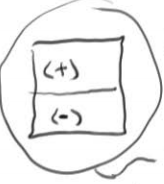
\includegraphics[height=100pt]{phases}
	\caption{The phases in the system. The extensive variables are Area, Volume, $\left\{ n_c \right\}$ (mole number or amount)}
      \end{figure}
      
      
      We still need $f = c - p + 2 = c$, from the phase rule, but $-A\d\gamma$ has $c+2$ variables! Therefore, we need two constraint formulas
      \begin{align}
	-A\d\gamma = S \d T - V\d P + n_{\ce{H2O}}\d\mu_{\ce{H2O}} + n_\ce{SDS} \d\mu_\ce{SDS}
	\tag{***}\label{Eq:base}
      \end{align}
      Find two side conditions for this example

      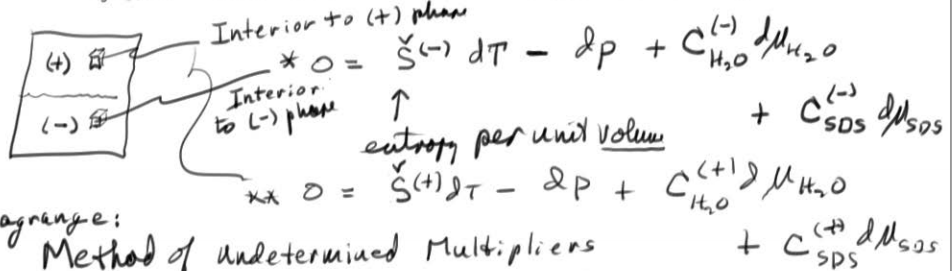
\includegraphics[height=100pt]{equationPicture}
      \begin{align}
	0 &= \check{S}^{(-)} \d T - \d P + C^{(-)}_\ce{H2O} \d\mu_\ce{H2O} + C^{(-)}_\ce{SDS}\d\mu_\ce{SDS}\tag{*}\label{Eq:+}\\
	0 &= \check{S}^{(+)} \d T - \d P + C^{(+)}_\ce{H2O} \d\mu_\ce{H2O} + C^{(+)}_\ce{SDS}\d\mu_\ce{SDS}\tag{**}
	\label{Eq:-}
      \end{align}
      \begin{subsection}{Lagrange: Method of undetermined multipliers}
      Multiply \eqref{Eq:+} by $\lambda^-$, \eqref{Eq:-} by $\lambda^+$ 
      Then subtract from \eqref{Eq:base} to obtain:
      \begin{align*}
	-A\d\gamma = (S - \lambda^{(+)}\check S^{(+)} - \lambda^{(-)}\check S^{(-)})\d T - (V-\lambda^{(+)}-\lambda^{(-)})\d P + \sum_{c=1}^{N}(n_c-\lambda^{(+)}C_c^{(+)}-\lambda^{(-)}C_c^{(-)})\d\mu_c
      \end{align*}
      Define:
      \begin{align*}
	\bar{S} &= \frac{1}{A}(S-\lambda^{(+)}\check S^{(+)}-\lambda^{(-)} \check S^{(-)})\\
	A &= \text{Area of the interface}\\
	\tau &= \frac{1}{A}(V - \lambda^{(+)} - \lambda^{(-)})\\
	\Gamma_\ce{H2O} &= \frac{1}{A}(n_\ce{H2O}-\lambda^{(+)}C_\ce{H2O}^{(+)} - \lambda^{(-)}C^{(-)}_\ce{H2O})\\
	\Gamma_\ce{SDS} &= \frac{1}{A}(n_\ce{SDS}-\lambda^{(+)}C_\ce{SDS}^{(+)} - \lambda^{(-)}C^{(-)}_\ce{SDS})\\
	\therefore -\d \gamma &= \bar{S}\d T - \tau \d P + \Gamma_\ce{H2O} + \Gamma_\ce{SDS}
      \end{align*}
      Each property is an ``Excess''
      Now, after Gibbs:
      Eliminate the pressure term and the water term, that is
    Take $\tau = 0, \Gamma_{H2O} = 0$ to define $\lambda^{(+)},\lambda^{(-)}$. This gives:
    \begin{align*}
    \begin{pmatrix}
      1 & 1\\
      C^{(+)}_\ce{H2O} & C^{(-)}_\ce{H2O}
    \end{pmatrix}
  \begin{pmatrix}\lambda^{(+)}\\ \lambda^{(-)}\end{pmatrix} = \begin{pmatrix}V\\n_\ce{H2O}\end{pmatrix}
  \end{align*}
  the solution of $\lambda^{(+)},\lambda^{(-)}$ can be determined by measured quantities through matrix inversion.
\end{subsection}
\begin{subsection}{$\d\gamma$}
  \begin{align*}
    -\d\gamma = \bar{S}\d T + \Gamma_\ce{SDS} \d\mu_\ce{SDS}
    \label{Eq:Gibbs Hansen formula for dgamma}
  \end{align*}Note the sign!

  We can measure $T, \mu_\ce{SDS}, \gamma$, so that, for example, at constant $T$
  \begin{figure}[h]
    \begin{subfigure}[t]{0.5\textwidth}
    \centering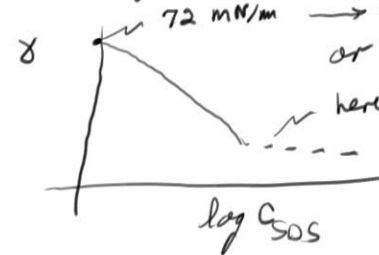
\includegraphics[height=100pt]{gammaVConcentration}
\caption{Ideal}
\end{subfigure}
\begin{subfigure}[t]{0.5\textwidth}  
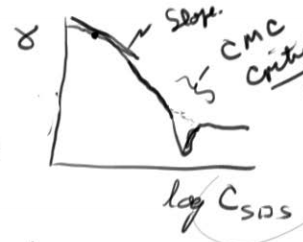
\includegraphics[height=100pt]{realitygammaVConcentration}
\caption{Most systems}
\end{subfigure}
\caption{Sketches of surface tension vs concentration at constant Temperature. The units of $\gamma$ are milliNewtons per meter, or milliJoules per meter$^2$. Note that the critical micellar concentration, CMC, introduces strange effects in the real system. Also note that above the CMC, the surface tension is independent of concentration. This is because the interface is saturated. The surfactant is usually not pure, which contributes to non-idealities of the system.
}
    \end{figure}
  \begin{align*}
    \mu_\ce{SDS} &= \mu_\ce{SDS}^{\deg} + RT\log{ (a_\ce{SDS})}\\
    a_\ce{SDS} &= \alpha(C_\ce{SDS})C_\ce{SDS} 
  \end{align*}
  Under certain conditions (when $C$ is small) $\alpha \rightarrow 1$

  Note: There may be cases where $\Gamma < 0$
  

  at constant $T$:
  \begin{align*}
    -\d\gamma = \Gamma_\ce{SDS}\d\mu_\ce{SDS}\\
    -\pOne{\gamma}{\mu_\ce{SDS}} = \Gamma_{SDS}
  \end{align*}
  after the critical micellar concentration (CMC) $\pOne{\gamma}{\mu}\approx 0$ so that the interface is saturated - $\Gamma_\mathrm{max}$

\end{subsection}
\end{section}
\begin{section}{Constant T}
  Consider 
  \begin{align*}
    \d\gamma = - \Gamma_\ce{SDS} \d\mu_\ce{SDS}
  \end{align*}

  What about an \underline{\underline{isotherm}}? You want a relation between $\Gamma_\ce{SDS},\mu_\ce{SDS} $ or $C_\ce{SDS}$ one would like 
  \begin{align*}
    \mu_\ce{SDS} &= \mu\deg + RT \log{(a)}\\
    a &= \alpha C\\
    \gamma &= \gamma_0 + f(\mu_\ce{SDS})
  \end{align*}
  However: Langmuir adsorption isotherm
  \begin{figure}[h]
    \centering
    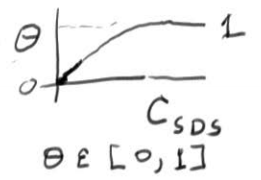
\includegraphics[height=100pt]{adsorptionIsotherm}
    \caption{A typical plot of the Langmuir adsorption isotherm}
    \label{fig:Langmuir}
  \end{figure}
  \begin{align*}
    \Theta = \frac{\Gamma_\ce{SDS}}{\max(\Gamma_\ce{SDS})}= \frac{\beta C_\ce{SDS}}{1+\beta C_\ce{SDS}}
  \end{align*} $\beta$ is sometimes called the ``Henry's law constant.''
  \begin{align*}
    -\d \gamma = \bar{S}\d T - \tau \d P + \sum_{c=1}^{N}\Gamma_c \d \mu_c
  \end{align*}
\end{section}
For example, consider: 
\begin{align*}
  \frac{\text{Oil Phase}}{\text{Water}} = \frac{\text{Major Phase}}{\text{Major phase}}
\end{align*}
Hansen's convention says $\Gamma_\text{water} = 0, \Gamma_\text{oil}=0$ so as to determine ($\lambda^{(+)}, \lambda^{(-)}$)
\begin{align*}
  -\d\gamma = \bar{S}\d T- \tau\d P + \sum_{c=3}^{N}\tau_c\d \mu_c\\
  \left( \pOne{\gamma}{P} \right)=\tau \stackrel{\mathclap{\normalfont\mbox{units of}}}{\:\:\:\:[=]\:\:\:\:} \si{L}
\end{align*}

$\tau$ is the ``interfacial excess of volume per unit area''

\begin{align*}
  \tau = \frac{1}{A}(V_\text{total} - (\lambda^{(+)} + \lambda^{(-)})) \text{so that for hansen}\\
  \lambda^{(+)} + \lambda^{(-)} \neq \text{total volume}
\end{align*}

\begin{section}{Interfacial region}
  \begin{figure}[h]
    \centering
    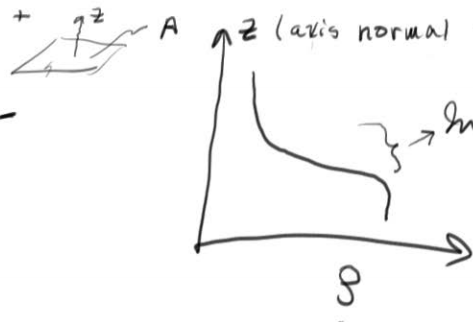
\includegraphics[height=100pt]{interfacialRegion}
    \label{fig:InterfacialRegion}
    \caption{The brackets denote the interfacial region. This is where the density has the biggest change over a small $\d z$. Note that $z$ is defined as being normal to the interface}
  \end{figure}
  Interfacial region - takes us to the ``Gibbs Surface'' construction, which I will do next time.
  \begin{figure}[h]
    \centering
    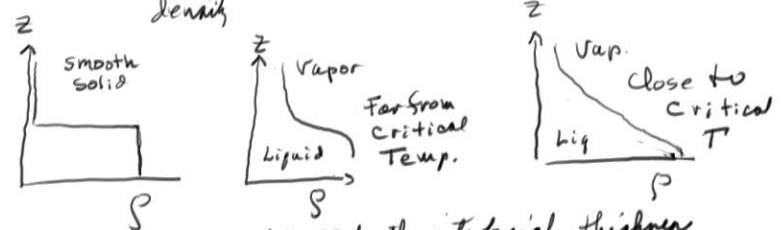
\includegraphics[height=100pt]{interfaceBar}
    \caption{Left: Smooth solid, interfacial thickness is very small. Middle: Vapor/liquid system far from the critical point, note the similarity to a $\tanh$. Right: Vapor/liquid system near the critical point. Note the large interfacial thickness and smooth variation in density}
    \label{fig:InterfaceBar}
  \end{figure}
  
Another way of stating Figure \ref{fig:InterfaceBar} is: Let $\xi$ be the interfacial thickness:
\begin{align*}
\xi\rightarrow\infty \text{ as } T\rightarrow T_\text{critical}
\end{align*}
\end{section}
\end{document}
